\documentclass[
    11pt,
    a4paper,
    sfdefaults=false,
    toc=chapterentrywithdots,
    oneside,openany,
    titlepage,
    parskip=half,
    headings=normal,  % reduces heading size
    listof=totoc,
    bibliography=totoc,
    index=totoc,
    captions=tableheading,  % caption below table
    chapterprefix=false,
    listof=flat,
    final
]{scrbook}


% details about your thesis
\newcommand{\titel}{Docker Swarm Mode}
\newcommand{\artderarbeit}{Hausarbeit f\"ur ``Cloud Native Computing'' \\}  % {Bachelorarbeit,Masterarbeit}
\newcommand{\autor}{Luise Hartdegen}
\newcommand{\studiengang}{Medieninformatik}  % {Informatik,Wirtschaftsinformatik,Medieninformatik}
\newcommand{\matrikelnr}{3642168}
\newcommand{\erstgutachter}{-}
\newcommand{\zweitgutachter}{-}
\newcommand{\betreuer}{Dr. Sven S\"ohnlein}
\newcommand{\unternehmen}{/}
\newcommand{\logo}{figures/TH-Nuernberg-RGB.png}
\newcommand{\keywords}{-}
\newcommand{\semester}{Wintersemester 2024/2025}
\newcommand{\abgabedatum}{TODO}

% custom head and foot
\usepackage[automark]{scrlayer-scrpage}
\pagestyle{scrheadings}
\ihead{\headmark}
\chead{}
\ohead{\pagemark}
\renewcommand*\chaptermarkformat{\chapappifchapterprefix{\ }% 
  \thechapter.\enskip}

\RedeclareSectionCommand[tocindent=0pt]{section}
\RedeclareSectionCommand[tocindent=0pt]{subsection}
%\RedeclareSectionCommand[tocnumwidth=70pt]{chapter}

\usepackage{scrhack}

% other packages
\usepackage[utf8]{inputenc}
\usepackage[T1]{fontenc}
\usepackage{lmodern,relsize,textcomp,csquotes}
\usepackage{amsmath,amsfonts}
\usepackage[ngerman]{babel}  % add english for english version
\usepackage[final]{graphicx}
\usepackage{setspace,geometry,xcolor}
\usepackage{makeidx}
\usepackage{paralist,ifthen,todonotes}
\usepackage{url}
\usepackage[toc]{glossaries}
\usepackage{pdfpages}

% table setup
\usepackage{longtable}
\usepackage{array}
\usepackage{ragged2e}
\usepackage{lscape}

% pdf hyperref
\usepackage[
    bookmarks=true,
    bookmarksopen=true,
    bookmarksnumbered=true,
    bookmarksopenlevel=1,
    pdftitle={\titel},
    pdfauthor={\autor},
    pdfcreator={\autor},
    pdfsubject={\titel},
    pdfkeywords={\keywords},
    pdfpagelabels=true,
    colorlinks=true,
    linkcolor=red,
    urlcolor=magenta,
    anchorcolor=black,
    citecolor=cyan,
    filecolor=magenta,
    menucolor=red,
    plainpages=false,
    hypertexnames=true,
    linktocpage=true,
]{hyperref}


% configure your listings style
\usepackage{listings}
\lstset{
	tabsize=3,
	extendedchars=true,
	frame=single,
	showstringspaces=true,
	numbers=left,
	numberstyle=\small,
	breakautoindent=true,
  basicstyle=\small,
  breaklines=true
}

% page setup
% \setlength{\topskip}{\ht\strutbox}
\geometry{paper=a4paper,left=2.5cm,top=3.0cm,bindingoffset=.8cm}
\onehalfspacing
\frenchspacing
\clubpenalty=10000
\widowpenalty=10000 
\displaywidowpenalty=10000

% some commands
\newcommand{\ua}{\mbox{u.\,a.\ }}
\newcommand{\zB}{\mbox{z.\,B.\ }}
\newcommand{\dahe}{\mbox{d.\,h.,\ }}
\newcommand{\bzw}{\mbox{bzw.\ }}
\newcommand{\bzgl}{\mbox{bzgl.\ }}
\newcommand{\eg}{\mbox{e.\,g.\ }}
\newcommand{\ie}{\mbox{i.\,e.\ }}
\newcommand{\wrt}{\mbox{w.\,r.\,t.\ }}
\newcommand{\etal}{\mbox{\emph{et\,al.\ }}}


\begin{document}

\setcounter{secnumdepth}{3}  % numerate subsections
\setcounter{tocdepth}{2}  % ...but don't include them in toc

\frontmatter
\thispagestyle{empty}
\pdfbookmark[1]{Cover}{cov}
\begin{titlepage}

    \begin{center}

    \includegraphics[width=\linewidth]{figures/ohm-logo.png}\\[1cm]
    \LARGE{Fakultät Informatik}\\[2cm]

    \huge
    \textbf{\titel}\\[1cm]
    %
    \Large
    \artderarbeit~im Studiengang \studiengang\\[1cm]
    %
    \large
    vorgelegt von

    \Large
    \autor\\[0.5cm]
    \small
    Matrikelnummer \matrikelnr\\[2cm]

    \vspace*{\fill}

    \large
        \begin{tabular}{p{3cm}p{8cm}}\\
        % Erstgutachter:  & \quad \erstgutachter\\[1.2ex]
        % Zweitgutachter: & \quad \zweitgutachter\\[1.2ex]
        %discomment "Betreuer" and "Unternehmen" for a thesis in a company
        Betreuer: & \quad \betreuer\\
        %Unternehmen: & \quad \unternehmen
        \end{tabular}

        \end{center}

        \begin{center}
    \copyright\,\the\year
    \end{center}

\vspace{-0.5cm}
\singlespacing
\small
\noindent Dieses Werk einschließlich seiner Teile ist \textbf{urheberrechtlich geschützt}.
Jede Verwertung außerhalb der engen Grenzen des Urheberrechtgesetzes ist ohne Zustimmung des Autors unzulässig und strafbar.
Das gilt insbesondere für Vervielfältigungen, Übersetzungen, Mikroverfilmungen sowie die Einspeicherung und Verarbeitung in elektronischen Systemen.

\end{titlepage}

% \cleardoublepage

% TODO download the following form (requires VPN) and complete it (hit save in your editor)
% https://intern.ohmportal.de/fileadmin/Public_Docs/SB/SB_0009_FO_Pruefungsrechtliche_Erklaerung_und_Erklaerung_zur_Veroeffentlichung_der_Abschlussarbeit_public.pdf
%\includepdf{SB_0009_FO_Pruefungsrechtliche_Erklaerung_und_Erklaerung_zur_Veroeffentlichung_der_Abschlussarbeit_public.pdf}\cleardoublepage

% \thispagestyle{empty}
\section*{Kurzdarstellung}
\label{sec:kurzdarstellung}
Kurze Zusammenfassung der Arbeit, höchstens halbe Seite.
Deutsche Fassung auch nötig, wenn die Arbeit auf Englisch angefertigt wird.

% \blindtext


\section*{Abstract}
\label{sec:abstract}
\emph{Only if thesis is written in English.}

% \blindtext
\cleardoublepage

\tableofcontents

\mainmatter
\chapter{Einführung}\label{ch:intro}

Motivation + Kurzfassung des restlichen Dokuments


% You may have read about similar things in \cite{Goodliffe2007}.
% You can also write footnotes.\footnote{Footnotes will be positioned automatically.}
% \blindtext

% \blindtext

% \section{This is an Important Section}

% It is possible to reference glossary entries as \gls{library} as an example.
% \blindtext

% \subsection{And an even more important subsection}
% \blindtext

\chapter{Technologie}\label{ch:technology}

Um die Verwendungszwecke von Docker Swarm näher zu untersuchen, muss zunächst die grundlegende Technologie grob erläutert werden. 
Docker ist an sich eine open-source ``platform for developing, shipping, and running applications''\cite{DockerInc} und besteht aus mehreren Komponenten. 

\section{Architektur}

Aufgebaut ist Docker nach der Client-Server-Architektur. Der Client kann hierbei jede Maschine sein, auf der Docker oder Docker Compose installiert ist und die docker-Befehle ausf\"uhren kann. 
Auf der Server-Seite steht dem gegen\"uber der Docker Daemon, der die eigentlichen Aufgaben des Bauens und Auslieferns \"ubernimmt. 
Ein Client kann dabei mit mehreren Daemons \"uber die Docker API kommunizieren. 

\begin{figure}[h]
    \centering
    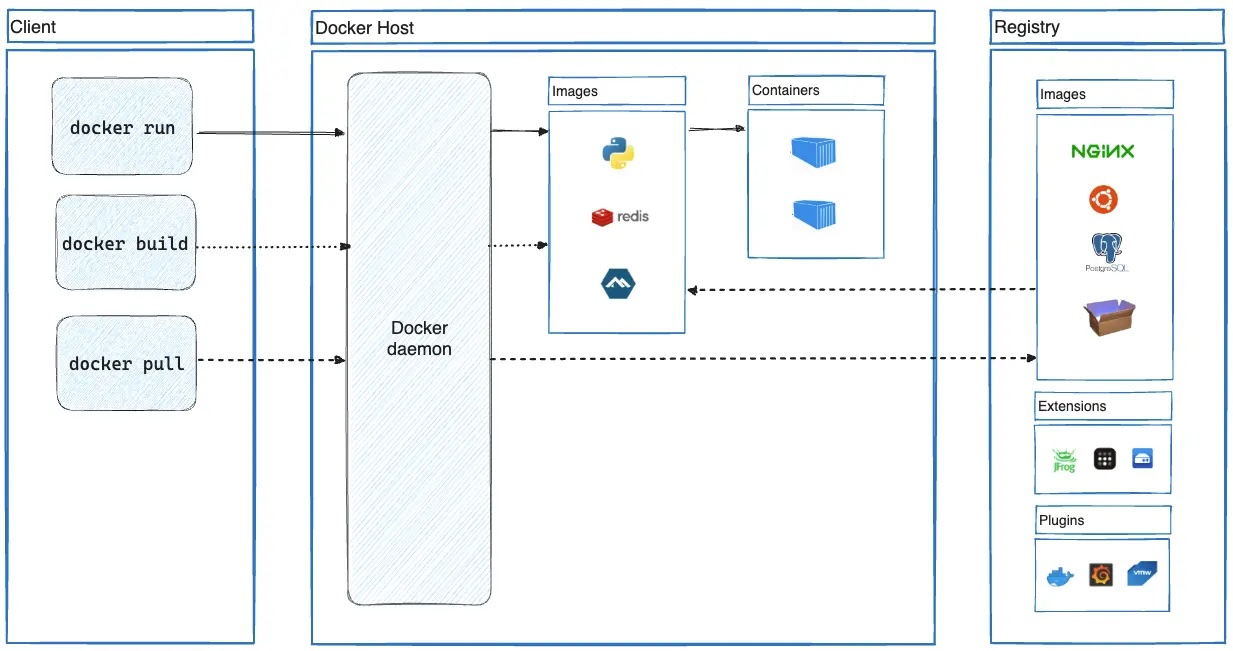
\includegraphics[width=0.7\textwidth]{figures/docker-architecture.jpeg}
    \caption{Aufbau der Docker-Architektur\cite{DockerInc}}
    \label{fig:docker-architecture}
\end{figure}

F\"ur Enduser-Betriebssysteme ist hier die Docker Desktop-Software relevant, die den Client, Daemon, Docker Compose  und weitere hilfreiche Komponenten mit einer graphischen Oberfl\"ache zusammen verpackt. 
Die dritte wesentliche Rolle neben Client und Daemon spielen die sogenannten Docker Registries, in denen Docker Images gespeichert werden. 
Docker selbst stellt eine \"offentliche Registry zur Verf\"ugung, das Docker Hub, in der viele offizielle Images wie bspw.\ die Base-Images f\"ur Datenbanken wie postgres, Reverse Proxys wie traefik oder auch simple Testimages wie hello-world zu finden sind. 
Dar\"uber hinaus kann jeder registrierte User dort kostenlos ein privates Repository sowie unbegrenzt viele \"offentliche Repositories f\"ur eigene Images erstellen. 
Unternehmen und Hochschulen verwenden hingegen in der Regel ein eigenes privates Registry, wenn die Images der Allgemeinheit nicht (kostenlos) zur Verf\"ugung gestellt werden soll.

Im Folgenden sollen zwei essentielle Aspekte beleuchtet werden; zum einen der grundlegende Aufbau und die Funktionalit\"at von Docker Containern und zum anderen das Konzept der Containerorchestrierung.

\section{Docker Container}

Docker Container basieren auf der Linux Container-Technologie und stellen eine Abstraktionsebene der klassischen Infrastruktur dar. 
W\"ahrend sie theoretisch als Alternative zur herkömmlichen Virtualisierung von Servern zum Einsatz kommen k\"onnen, werden diese beiden Technologien in der Praxis meist kombiniert. 
Das Ziel ist dabei, eine Umgebung zu schaffen, die dem gewünschten Betriebssystem möglichst nah kommt, ohne einen separaten Kernel zu benötigen\cite{quan_connecting_2016} und dabei gleichzeitig leichtgewichtig und portabel genug zu sein, um jederzeit schnell und bestenfalls automatisiert ersetzt werden zu k\"onnen. 
Container verpacken Software in einem vollständigen Dateisystem, das alles beinhaltet, was gebraucht wird, um die Software zuverlässig und konsistent  auszuführen. 
Das umfasst sowohl den Code als auch die Laufzeitumgebung, Bibliotheken und weitere Abhängigkeiten.\cite{nguyen_distributed_2017}
Sie bestehen also ``aus einem oder mehreren Prozessen, die vom Rest des Systems isoliert sind''.\cite{red_hat_was_2023}
Die Isolation des Codes gegen\"uber anderen Containern auf dem gleichen System wird gew\"ahrleistet, indem die Docker Engine f\"ur jeden Container einen eigenen Namespace erstellt, an den alle Aspekte des Containers gebunden sind.\cite{DockerInc}
Im Gegensatz zu Kubernetes findet dies aber nur intern statt und wird nicht durch die Anwenderin direkt beeinflusst. 

\begin{figure}[h]
    \centering
    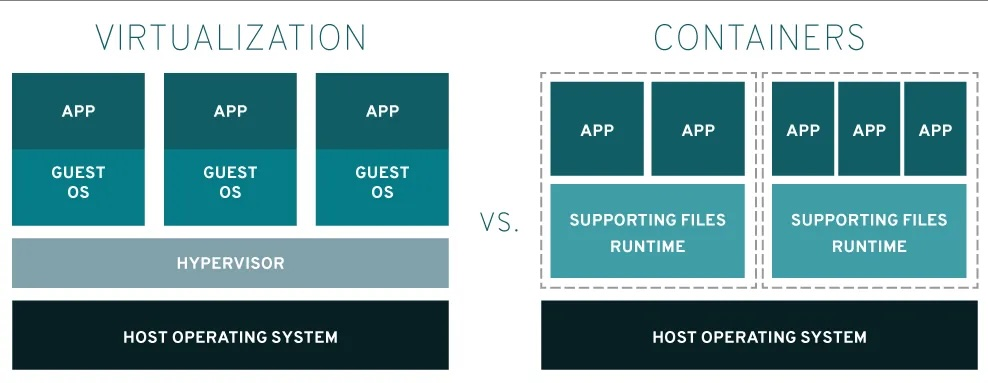
\includegraphics[width=0.7\textwidth]{figures/virtualization-vs-containers.jpeg}
    \caption{Vergleich von Virtualisierung und Containerisierung\cite{red_hat_was_2023}}
    \label{fig:virtualization-comparison}
\end{figure}

Im Gegensatz zur Virtualisierung, bei der für jede virtuelle Maschine ein eigenes Betriebssystem installiert wird, verwendet die Containerisierung das Betriebssystem des Hosts, wodurch die Container leichtgewichtiger und portabler sind. 
Im Umkehrschluss bedeutet das aber auch, dass ein Container immer nur auf dem Betriebssystem laufen kann, für das er gebaut wurde. 
So kann ein Container mit einer zugrunde liegenden ARM-Architektur nicht auf einem x86 Linux-System laufen und umgekehrt. 
Da es aber möglich ist, die Zielarchitektur beim Erstellen zu definieren, stellt dies in der Praxis kein echtes Problem dar.

\section{Docker Images}

``Alle zur Ausführung [eines Containers] notwendigen Dateien werden über ein eigenes Image bereitgestellt''\cite{red_hat_was_2023}, das in einer Textdatei namens Dockerfile beschrieben ist. 
Das Image stellt somit eine Vorlage für die einzelnen Container dar, die die Docker Engine instanziiert. 
Es basiert in der Regel auf einem vorgefertigten Image, wie bspw.\ node als Laufzeitumgebung zum Bauen des Codes und nginx als Webserver zum Ausliefern im Codebeispiel~\ref{lst:Dockerfile}.
Die Datei besteht aus Instruktionen, die sequentiell abgearbeitet werden, wobei jede Instruktion ein Layer des Images erstellt.
Daher werden beim Bauen eines Images nur diejenigen Layer neu gebaut, in denen sich etwas ge\"andert hat.

\lstinputlisting[language=bash,caption={Codebeispiel eines Dockerfiles},captionpos=b,label=lst:Dockerfile]{listings/Dockerfile}

Wird nun auf Basis des erstellten Images ein Container erstellt, verändern die Instruktionen das Dateisystem der jeweiligen Laufzeitumgebung, aber immer nur in Bezug auf den Namespace des Containers. 

\chapter{Docker Swarm}\label{ch:dockerswarm}

Nachdem ein Dockerfile für einen Microservice erstellt und das Image gebaut wurde, ist der nächste Schritt das Ausliefern der Software. 
Während Docker Container lokal zum Testen problemlos einzeln über die Kommandozeile oder auch als Gesamtpaket per Docker Compose-Datei gestartet werden können, ist dies für Test- und Produktivumgebungen mühselig und unpraktikabel zu pflegen. 
Die Container einmalig zu starten, ist schließlich nur der Anfang.
H\"aufig besteht eine Software aus mehreren Microservices, die \"uber mehrere Hosts verteilt sind. 
Über die Lebensdauer einer Software hinweg, muss kontrolliert werden, ob der Container fehlerfrei läuft und dass er nicht abstürzt, um die Verfügbarkeit zu gewährleisten.
Unter Umständen müssen mehrere Container-Instanzen gestartet werden, um einer höheren Last standhalten zu können. 
Zudem muss die Kommunikation zwischen einzelnen Containern und zwischen Containern und der Außenwelt sichergestellt werden. 

All diese Punkte ergeben zusammen die sogenannte Containerorchestrierung. 
Diese Tätigkeit kann manuell ausgeführt werden, aber im Zeitalter der Automatisierung und DevOps-Kultur gibt es dafür selbstverständlich bessere Optionen. 
Am weitesten verbreitet ist hierbei das System Kubernetes, das von Google entwickelt wurde, aber schon von Anfang an der Community als Open-Source-Projekt zur Verfügung gestellt wurde. 
Es dient der automatisierten Bereitstellung, Skalierung und Verwaltung von containerisierten Anwendungen, bietet aber darüber hinaus viele weitere Optionen.

Entsprechend ist die Software recht komplex und kann anfangs inbesondere f\"ur Einsteigerinnen eine Herausforderung darstellen. 
Alternativ dazu gibt es eine hauseigene Plattform zur Containerorchestrierung von Docker selber, den Docker Swarm Mode. 
Ein Swarm ist ein Cluster bestehend aus einer oder mehrerer Docker Engines verteilt auf mehreren Servern oder virtuellen Maschinen.\cite{Docker_Engine_Swarm}
Der Docker Swarm Mode ist seit 2016 nativ ein Teil von Docker, aber standardm\"a{\ss}ig ausgeschaltet.
Der folgende Abschnitt beleuchtet den Aufbau und die Funktionsweise dieser Plattform.  

\section{Nodes}

Die einzelnen Docker Engines, die Teil eines Swarms sind, werden als Nodes bezeichnet. 
Jede Node hat zur Laufzeit entweder die Rolle eines Managers oder Workers, wobei die Rollen dynamisch durch User ge\"andert werden k\"onnen. 

Ein Manager-Node ist daf\"ur zust\"andig, mithilfe des Raft-Algorithmus den internen Zustand des Swarms zu erhalten, also bswp.\ die Anzahl an definierten Containern eines bestimmten Services sicherzustellen und einen neuen Container hochzufahren, wenn einer fehlschl\"agt. 
Dar\"uber hinaus \"ubernimmt der Manager Scheduling-Aufgaben und stellt die HTTP API-Endpunkte des Swarms bereit. 
Im Gegensatz dazu ist die einzige Aufgabe eines Worker-Nodes, die Container gem\"a{\ss} den spezifizierten Instruktionen auszuf\"uhren. 

Jeder Manager-Node ist immer gleichzeitig auch ein Worker-Node, weshalb ein Swarm aus genau einem Manager-, aber niemals aus nur einem Worker-Node bestehen kann. 
Um die Fehlertoleranz des Swarm Modes effektiv nutzen zu k\"onnen, wird empfohlen, einen Swarm aus einer ungeraden Anzahl $N$ an Manager-Nodes aufzubauen. 
Dadurch kann der Verlust von $\frac{N-1}{2}$ Manager-Nodes toleriert werden und der Swarm erholt sich ohne Downtime. 
Docker empfiehlt ein Maximum von sieben Manager-Nodes, da potentiell eine h\"ohere Anzahl an Managers die Performanz reduziert.\cite{Docker_Engine_Nodes}

\begin{figure}[h]
    \centering
    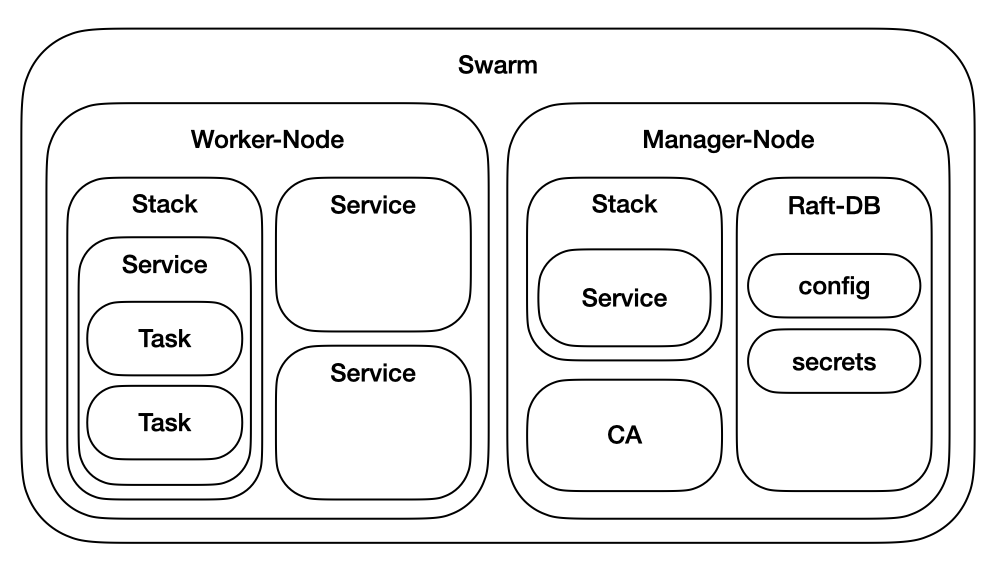
\includegraphics[width=0.7\textwidth]{figures/SwarmArchitecture.png}
    \caption{\"Ubersicht des architektonischen Aufbaus eines Docker Swarms}
    \label{fig:docker-swarm-architecture}
\end{figure}

\section{Services und Tasks}

Eine weitere logische Einheit in einem Docker Swarm nach den Nodes sind die Services. 
Diese sind oft einzelne Microservices im Kontext einer gr\"o{\ss}eren Anwendung, z.B.\ das Front- und Backend einer Anwendung oder auch eine Datenbank. 
Wie im Codebeispiel~\ref{lst:Compose} gezeigt, wird ein Service \"uber einen Namen (``frontend'') definiert und das zu verwendende Image angegeben. 
Alle weiteren Angaben sind optional, dazu z\"ahlt unter anderem
\begin{itemize}
    \item das Netzwerk, um mehrere Services untereinander erreichbar zu machen,
    \item Unter- und Obergrenzen bez\"uglich der Hardware-Ressourcen und 
    \item der gew\"unschte Zustand des Deployments, wie die Anzahl an Replikas und unter welchen Bedingungen ein Service neugestartet werden soll.
\end{itemize}

Wenn ein so definierter Service in einem Swarm ausgeführt wird, werden diese Angaben in die Raft-Datenbank der Manager-Nodes \"ubernommen, damit diese von dem Moment an den sogenannten Desired State umsetzen k\"onnen.
Das bedeutet, dass der zust\"andige Manager f\"ur jede geforderte Replika einen Task startet, der einen Container nach den genannten Vorgaben hochf\"ahrt. 
Ein Task ist somit die kleinste Verwaltungsstruktur im Docker Swarm, die genau einen Container enth\"alt und neu gestartet wird, wenn der Container den Anforderungen in der Service-Definition nicht mehr gen\"ugt, also z.B.\ wenn der Container abst\"urzt.
Die Tasks werden auf die verf\"ugbaren Worker-Nodes je nach deren Auslastung verteilt.\cite{Docker_Engine_Services}

\lstinputlisting[language=bash,caption={Compose-File zur Auslieferung eines Frontend-Services als Stack},captionpos=b,label=lst:Compose]{listings/docker-compose.yaml}

\section{Deklarativer Ansatz}

Um den gew\"unschten Zustand der Services innerhalb eines Swarms festzulegen, verwendet die Docker Engine einen deklarativen Ansatz. 
Das bedeutet, dass ein Service innerhalb einer Compose-Datei, in der Regel als yaml, definiert wird. 
In dieser Datei stehen alle Informationen, die der Manager-Node ben\"otigt, um den Service zu starten und bei Bedarf zu reparieren. 
Zu beachten ist dabei, dass die Compose-Datei im Legacy-Format Compose file version 3 sein muss, wenn der Service als Stack ausgeliefert werden soll. 
Ein Stack dient dabei der einfacheren Auslieferung von mehreren Services als Gesamtpaket und ist vergleichbar mit Docker Compose f\"ur die lokale Entwicklung.\cite{Docker_Engine_deploy}
\chapter{Vergleich zwischen Docker Swarm und Kubernetes}\label{ch:comparison}

Wie eingangs bereits erw\"ahnt, ist Docker Swarm nicht die einzige Software zur Containerorchestrierung.
Neben anderen Alternativen gibt es Kubernetes, das nicht nur bekannter und weiter verbreitet ist, sondern inzwischen auch direkt in Docker Desktop integriert ist und den Industriestandard darstellt. 
Ohne zu tiefgreifend auf die Architektur und Funktionsweise von Kubernetes einzugehen, soll dennoch im Folgenden ein Vergleich zwischen den beiden Optionen gewagt werden.

\begin{figure}[h]
    \centering
    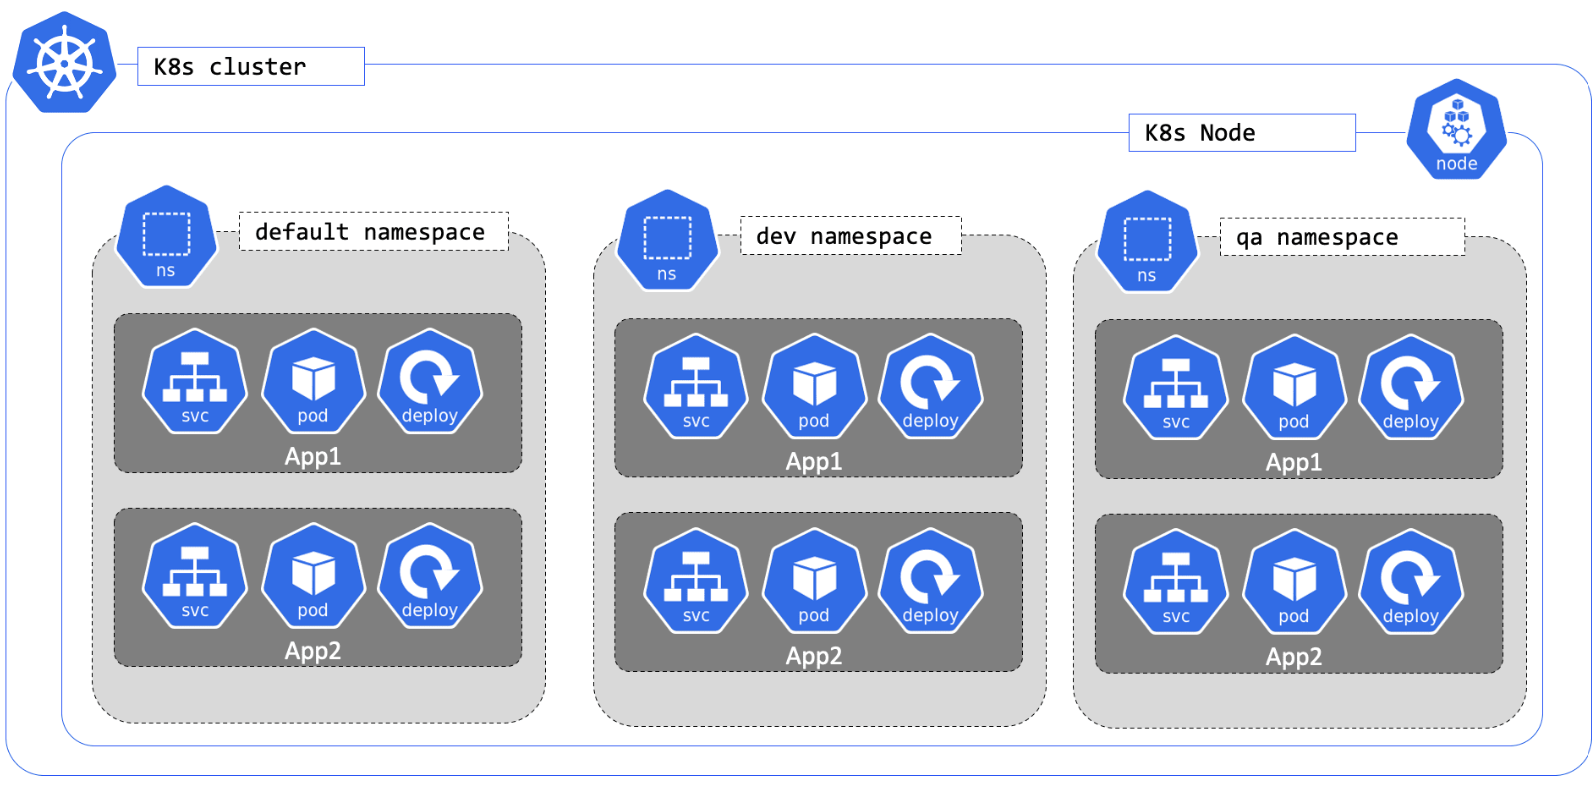
\includegraphics[width=0.7\textwidth]{figures/kubernetes.png}
    \caption{\"Ubersicht des architektonischen Aufbaus eines Kubernetes-Clusters\cite{kumar_working_2019}}
    \label{fig:k8s-cluster}
\end{figure}

In den Grundfunktionalit\"aten unterscheiden die beiden Orchestrierungssoftwares sich wenig. 
Sie beinhalten gleicherma{\ss}en Funktionen, um Docker Container zu starten, zu stoppen, deren Verf\"ugbarkeit zu kontrollieren und auf Ausf\"alle zu reagieren. 
Ebenso bieten beide Systeme Optionen zur Lastverteilung und Ressourcenverwaltung des Host-Systems. 
Dadurch k\"onnen z.B.\ Container automatisiert von einem System auf ein anderes im gleichen Cluster umgezogen werden, sofern ein Cluster Fehler wirft oder nicht mehr gen\"ugend Ressourcen bereitstellen kann. 

In der Art und Weise wie Skalierung gehandhabt wird, treten aber schon die ersten Unterschiede auf. 
Skalierung bezeichnet das Replizieren von Containern, um eine h\"ohere Last aufzufangen.
Bei Docker Swarm muss die Anzahl an Replikas immer manuell angegeben werden, entweder wie oben gezeigt \"uber die Compose-Datei, im Nachhinein durch einen Docker-Befehl oder eine separate UI wie bspw.\ Portainer. 
In Kubernetes hingegen ist es m\"oglich festzulegen, dass bspw.\ ab einer bestimmten Auslastung automatisch zus\"atzliche Container in sogenannten Pods gestartet werden. 
Dies geschieht mittels des Horizontal Pod Autoscalers (HPA), der ``die Anzahl der Pods in einem Deployment oder Replica Set basierend auf beobachteten CPU-Auslastung oder anderen ausgewählten Metriken automatisch skaliert''.\cite{briegel_kubernetes_2023}
Dies wird unterst\"utzt durch den Vertical Pod Autoscaler und den Cluster Autoscaler, die zus\"atzliche Skalierungsoptionen bieten.\cite{briegel_kubernetes_2023}

Ein Aspekt, der inbesondere im Kontext von cloud-basierten Anwendungen relevant ist, ist die Sicherheit. 
Hier bieten beide Systeme ihre eigenen L\"osungen an, wenn auch auf unterschiedliche Art und Weise. 
Der Netzwerkverkehr zwischen Containern ist in Docker Swarm standardm\"a{\ss}ig verschl\"usselt, um Man-in-the-Middle-Angriffe oder \"ahnliches zu verhindern. 
Dar\"uber hinaus stellt Docker Swarm grundlegende Funktionalit\"aten zur Verwaltung von Secrets zur Verf\"ugung. 
W\"ahrend diese Funktionen ohne Frage wichtig sind, sind bei Docker Swarm  die Konfigurationsoptionen diesbez\"uglich beschr\"ankt.

Das ist einer der Punkte, aufgrund dessen Kubernetes in vielen F\"allen bevorzugt wird. 
Nicht nur bietet Kubernetes diese beiden und mehr Funktionen an, sondern gibt den Userinnen auch mehr M\"oglichkeiten, bspw.\ Netzwerkrichtlinien auf der Ebene von Pods zu erstellen.\cite{briegel_kubernetes_2023}

% \chapter{Anwendungsf\"alle f\"ur Docker Swarm}\label{ch:usecase}

% \Blindtext

\chapter{Fazit}\label{ch:summary}

Zusammenfassend kann man sagen, dass Kubernetes zu Recht als De-facto-Standard im Bereich Containerorchestrierung gilt und eine enorme Bandbreite an Funktionen bietet. 
Jedoch geht diese Vielseitigkeit auch mit einer gewissen Einstiegshürde einher. 
Die Einrichtung und Verwaltung eines Kubernetes-Clusters erfordert tiefgehendes Wissen und ist insbesondere für kleinere Projekte mit zusätzlichem Aufwand verbunden.

Wer sich beruflich im Bereich der Containerorchestrierung weiterentwickeln möchte, sollte sich definitiv mit Kubernetes auseinandersetzen. 
Durch seine breite Verwendung in der Industrie und den hohen Funktionsumfang ist es eine essenzielle Technologie für DevOps- und Cloud-native Umgebungen.

Für viele Projekte, insbesondere im universitären oder experimentellen Umfeld, ist jedoch nicht immer eine so komplexe Lösung erforderlich. 
In Szenarien, in denen die Containerorchestrierung nur ein Aspekt unter vielen ist, bietet Docker Swarm eine deutlich einfachere Alternative mit niedrigeren Einstiegshürden, insbesondere wenn die beteiligten Personen sich bereits in Ans\"atzen mit Docker auseinander gesetzt haben. 
Auch für produktive Umgebungen, in denen eine schlanke und unkomplizierte Verwaltung ausreicht, kann Docker Swarm eine sinnvolle Wahl sein.

Letztlich hängt die Wahl des richtigen Orchestrierungswerkzeugs von den individuellen Anforderungen des Projekts ab. 
Während Kubernetes für großflächige, skalierbare Systeme die erste Wahl ist, kann Docker Swarm eine pragmatische Lösung für weniger komplexe Anwendungsfälle und Lernumgebungen darstellen.

\backmatter
\listoffigures
% \cleardoublepage

% \listoftables
% \cleardoublepage

\renewcommand{\lstlistlistingname}{Codebeispiele}  % change for German thesis
\lstlistoflistings%
% \cleardoublepage

% \bibliographystyle{wmaainf}
% \bibliography{refs}

\nocite{*}
\bibliographystyle{IEEEtran}
\bibliography{refs}

% remove if not needed
\appendix
\renewcommand{\appendixname}{Anhang}
\chapter{Anhang}\label{app:supplemental-information}

Es wurden keine KI-Tools zur Erstellung der vorliegenden Arbeit verwendet. 

% \printnoidxglossaries

\end{document}
